\documentclass[a4paper,10pt]{article}
\usepackage{amsmath}
\usepackage{amsthm}
\newtheorem{mydef}{Definition}
\usepackage{url, hyperref}
\usepackage{amsthm}
\usepackage{amsfonts}
\usepackage{amssymb}
\newtheorem{theorem}{Theorem}
\newtheorem{lemma}{Lemma}
\usepackage{fullpage}
\usepackage{tikz}
\usepackage{float}
\usepackage{listings}
\usepackage{color}
\bibliographystyle{plain}

\title{Vorderingsverslag 1: 'n Ondersoek na effektiewe segmenteringsalgoritmes vir gebruik in haaifin-identifikasie}
\author{L. Cilli\'{e}, 16010450}
\date{22 Februarie 2013}

\begin{document}
\maketitle
\section{Inleiding}
Gedurende die afgelope twee weke is 'n groot verskeidenheid areas ondersoek
en is daar nie net spesifiek op die projekonderwerp gefokus nie.  Daar is ondermeer na die volgende gekyk:
\begin{itemize}
 \item Die gebruik van Git en Github
 \item Die gebruik van IPython vir die vorderingsverslae asook die finale projekverslag
 \item Die installasie van nodige sagteware en opstel van die masjien
 \item Voorbeelde wat deel vorm van die Scikit-image pakket
 \item Artikels en webwerwe
 \item Data
\end{itemize}

\noindent Hierdie onderwerpe sal nou in meer besonderhede bespreek word.

\section{Bespreking}
\subsection{Die gebruik van Git en Github}
Git is kragtige, gratis en oopbron sagteware wat help met die kontrole van inligting, kode, webwerwe ens.  
Dit vergemaklik die proses waar verskeie persone bydraes maak tot 'n projek.  Kode word eenvoudig op die github
stelsel gelaai. Daarna kan die kode met ander gedeel word, verandering aangebring word en algemene opmerkings oor die kode gemaak word.
Dit is 'n kragtige stuk gereedskap ter ondersteuning van die projek. Sien \url{http://git-scm.com/} vir meer inligting.

\subsection{Die gebruik van IPython vir die vorderingsverslae asook die finale projekverslag}
Hoe werk die ipython notaboek?  Die ipython notabook is 'n interaktiewe, webgedrewe omgewing waar die loop van kode,
teks, grafieke, Wiskunde, ens. gekombineer kan word en as 'n enkele dokument saamgestel kan word. Hierdie dokumente kan ook met 
ander gedeel word en kan maklik in formate soos PDF omgeskakel word.  Dit neem onder andere \mbox{\LaTeX } kode in as toevoer.   Dit is 'n gerieflike en effektiewe manier om alle 
komponente van die projek te kombineer. Die notaboek sal vir die duur van die projek gebruik word. Sien \url{http://ipython.org/notebook.html} vir meer inligting.

\subsection{Die installasie van nodige sagteware en opstel van die masjien}
Verskeie pakkette soos git, python, ipython, ipython notebook, numpy, scipy, matplotlib, scikit-image en skimage word benodig om sommige van die 
algoritmes te kan loop.  Al bogenoemde is ge\"{i}nstalleer en ander algemene masjienprobleme is uitgesorteer. 

\subsection{Voorbeelde wat deel vorm van die Scikit-image pakket}
Scikit-image is 'n versameling van algoritmes (geskryf in python) wat in beeldverwerking gebruik word.  Dit is 'n gratis, oopbron pakket saamgestel
deur 'n groep vrywilligers. Verskeie segmenteringsalgoritmes in hierdie pakket is ondersoek om 'n 
basiese idee te kry van die werking daarvan en hoe scikit-image aanmekaargesit is. 
Byvoorbeeld, die \emph{Random Walker Segmentation} algoritme, \cite{scikit}, wat die volgende produseer:
\begin{figure}[H]
 \centering
 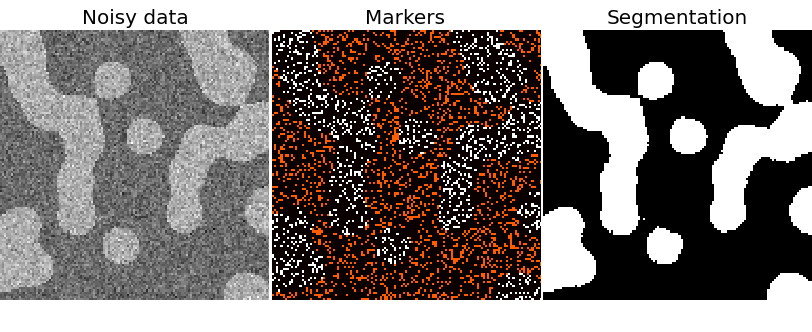
\includegraphics[width=5in, height=2in]{Verslag1_fig}
 \caption{Hierdie segmenteringsalgoritme maak gebruik van merkers wat verskillende fases in die beeld merk}
 \label{haai}
\end{figure}
\noindent Sien \url{http://scikit-image.org} vir meer inligting.

\subsection{Artikels en webwerwe}
Tans word \cite{art} bestudeer.  Dit is 'n oorsigartikel wat handel oor verskeie segmenteringsalgoritmes.  Daaruit word beoog om duidelikheid te kry oor die werking en kompleksiteit van bestaande effektiewe algoritmes.  Verskeie webwerwe in die 
verband is ook beskikbaar, soos byvoorbeeld \url{http://www.alphamatting.com/}.  Hierdie webwerf handel spesifiek oor die tegniek,
alpha matting, en vergelyk verskillende segmenteringsalgoritmes deur dit op beelde met spesifieke eienskappe toe te pas.  

\subsection{Data}
Verskeie voorlopige haaifinbeelde is as eksperiment gebruik. Soortgelyke beelde, sien Figuur 2, sal 'n integrale deel van die studie vorm.  
Hierdie beelde is in scikit-image ingelees en daar is gekyk na 
hoe die bestaande segmenteringsalgoritmes op die beelde werk.  Sommige van die algoritmes vereis ook dat bestaande voor- en agtergrond identifiseer word.  Dit kan vir eers gedoen word deur
die hoeke as agtergrond te merk en die middel-onder as voorgrond te merk.  Die proses word aansienlik vergemaklik deur die foto's wat reeds netjies 
uitgeknip is.
\begin{figure}[H]
 \centering
 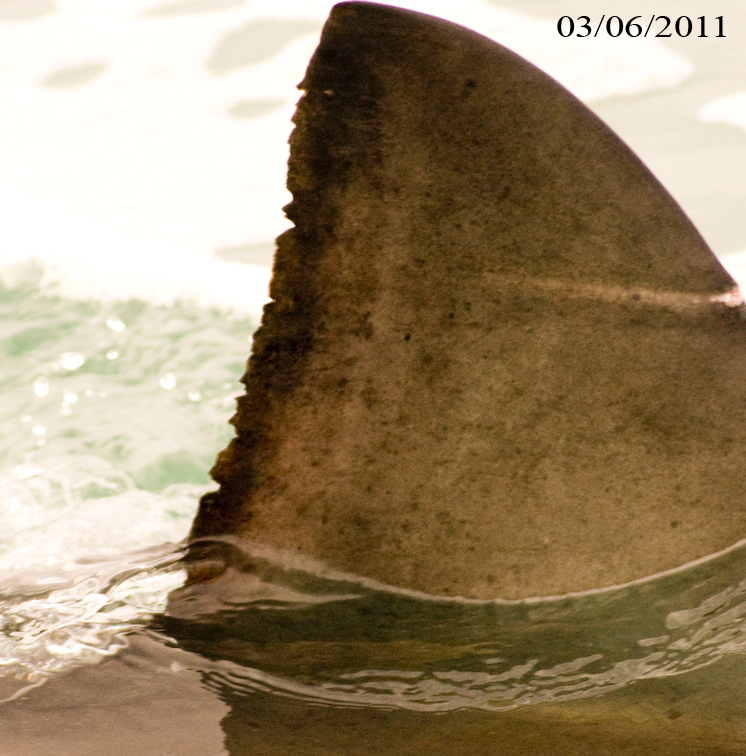
\includegraphics[width=2in, height=1.8in]{haai2}
 \caption{'n Voorbeeld van 'n haaifinbeeld}
 \label{fin}
\end{figure}

\section{Wat word beplan?}
Vir die volgende twee weke word die volgende beplan
\begin{itemize}
 \item Prof. Johan du Preez het 'n interessante segmenteringsalgoritme ontwerp wat gebou is op grafiese modelle.
 Dit gaan verder ondersoek word en hy het ges\^{e} dat hy die projek sal ondersteun.
 \item Lees \cite{art} klaar om duidelikheid te kry oor die werking en kompleksiteit van die algoritmes en te help om een van die beter, tog 
 eenvoudige algoritmes, te implementeer.
 \item Bestudeer die gekose bogenoemde algoritmes in diepte en pas dit op die haaibeelde toe om die effek te ondersoek.
 \item Raak vertroud met die betrokke sagteware wat die segmenteringsalgoritmes gebruik.
\end{itemize}

\newpage
\bibliography{V1}
\end{document}
